\documentclass[12pt,english]{report}
\usepackage[T1]{fontenc} % https://tex.stackexchange.com/questions/664/why-should-i-use-usepackaget1fontenc
\usepackage{babel} %https://tex.stackexchange.com/questions/27740/whats-the-benefit-of-loading-babel-when-writing-in-english
\usepackage{subcaption} % https://tex.stackexchange.com/questions/119984/subfigures-side-by-side-with-captions

%\usepackage[margin=1in]{geometry}
%\usepackage{enumitem}
%\usepackage{float}
%\usepackage{empheq}
%\usepackage{datetime}

\usepackage[shortlabels]{enumitem}
\usepackage{empheq}
\usepackage{url}
\usepackage{amsmath, amssymb}
\usepackage[export]{adjustbox} % also loads graphicx
\usepackage{textcomp}
\usepackage{color}
\usepackage{nicefrac}
\usepackage{cancel} % \cancel for strike through text but diagonal
\usepackage[normalem]{ulem} % for \sout strike through text

%\usepackage{steinmetz}
%\newcommand{\HW}{Hot Wheels\textsuperscript{\textregistered}}
\newcommand{\HW}{Hot Wheels}
%\newcommand{\Matchbox}{Matchbox\textsuperscript{\textregistered}}
\newcommand{\Matchbox}{Matchbox}

\newcommand{\revise}[1]{{\color{red}\textit{#1}}}
\newcommand*{\multicitedelim}{:}

\newcommand{\degree}{$^{\circ}$}
\newcommand{\degre}{^{\circ}}

\newcommand{\Ohm}{$\Omega$}

\newcommand{\Fbox}[1]{\fbox{$\displaystyle #1$}}

\newcommand{\ezfig}[2]{
\begin{figure}[t]
\centering
\includegraphics[width=\linewidth]{images/#1.png}
\caption{\label{fig:#1} #2}
\end{figure}
}

\newcommand{\ezfigstar}[2]{
\begin{figure*}[t]
\centering
\includegraphics[width=\linewidth]{images/#1.png}
\caption{\label{fig:#1} #2}
\end{figure*}
}

\newcommand{\code}[1]{{\fontfamily{pcr}\selectfont #1}}


\author{
	King, Jaiden\\
	\texttt{jaiden.king.035@my.csun.edu}
	\and
	Greeff, Guy\\
	\texttt{guy.greeff.241@my.csun.edu}
	\and
	Rojas, Richard\\
	\texttt{richard.rojas.717@my.csun.edu}
	\and
	Schnider, Nathan\\
	\texttt{nathan.schnider.455@my.csun.edu}
	\and
	Thomas, Ryan\\
	\texttt{ryan.thomas.732@my.csun.edu}
}
\title{
\includegraphics[width=0.2\linewidth]{images/CSUNS.png}\\
Trajectory Estimation of a Ballistic Projectile Experiencing Aerodynamic Drag\\\large{An Exercise in Modeling Our World}}

\begin{document}
\maketitle

\tableofcontents

% PLACEHOLDER IMAGE 
% This is just here to show how to include a graphic
\begin{figure}[t]
\centering
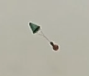
\includegraphics[width=0.5\linewidth]{images/BallMidFlight.png}
\caption{\label{fig:BallMidFlight} A photograph of our system. The system consists of a projectile traveling on an arc through the air after being thrown with some initial velocity. A drogue chute has been attached with the intention of linearly varying the aerodynamic drag, though it may have more dynamic impacts than intended.}
\end{figure}

% To reference the figure by number: Fig.~\ref{fig:BallMidFlight}

\section{Introduction}

The natural world is full of fascinating phenomena. Our ancestors have worked tirelessly to develop the language of mathematics to describe these phenomena. While exact analytic solutions to some of the more complicated problems often do not exist, or are too impractical to solve by hand, there are numerical techniques to approximate the solutions to these problems. However, the numerical techniques are still quite laborious to compute. Powerful institutions could employ teams of computers to labor for hours solving problems of science and engineering that we would find trivial today. 

We live in an exciting point in history where the profession of computer has been fully automated by machines. And not just automated for powerful institutions, but also made accessible to nearly all of humanity. The amount of compute accessible to anyone reading this paper is beyond the comprehension of our ancestors who originally developed the mathematics we shall employ. 

Modern hardware is capable of computing small models in what feels like an instant, and with these models we can foresee the future. As engineers, we must be comfortable wielding this immense power. 

In this paper we shall identify some physical phenomenon, develop a mathematical model of it, and develop computer software to compute the model.

\subsection{Selecting a Phenomenon}

We're interested in modeling a phenomenon which is simple enough in scope to implement over a couple weeks, but could be representative of some more complex system being used in the world today. 

Consider the phenomenon of an object flying through the air. A wide variety of applications depend on the ability to accurately predict the future location of such flying objects. Examples of automated computer systems tracking projectile objects are abundant in the fields of missile/drone guidance and missile/drone defense. Beyond automated systems, human minds have to compute trajectories in many scenarios. Many sports require throwing and catching balls, and even in agriculture there is a need to predict trajectories.

We're going to model an object traveling on a ballistic trajectory. We will take samples of the position of some object over time, then use those samples to fit a trajectory, then use that trajectory to predict where the object will impact the ground.


\section{Data Collection}
\section{System Identification}

Consider our system of a parachute attached to a spherical mass by a string being thrown through the air. How can we model this system? The answer may seem obvious depending on your physics background, but we claim that nothing is obvious.\footnote{Any problem worth studying will not have an obvious answer. If the answer seems obvious, question your assumptions.}

First it's important to identify what properties of the system we're actually interested in. Here we've decided we're interested in modeling the trajectory of the center of mass of the ball. Some things we aren't interested in are the motion of the parachute, the mass of the ball, the elasticity of the ball, the color of the ball, the temperature of the room, the location of the moon in relation to the Earth, what you had for breakfast, etc. 

Everything in the universe is connected\footnote{This is readily apparent by considering gravity or electromagnetism.} and where we choose to draw the line may seem arbitrary. Obviously we won't be modeling every atom of our system and all the forces they're experiencing, but there are still a handful of reasonable options:

\begin{enumerate}
\item Point Mass, No Drag\footnote{ADD FIGURE: Freebody diagram}

The ball-chute system could be modeled as a single point mass in a vacuum traveling on a parabolic trajectory. This would certainly miss 

\item Point Mass, Linear Drag\footnote{ADD FIGURE: Freebody diagram}



\end{enumerate}


\section{Computer Software Design}
\section{Results Analysis}

So how does the parabolic model perform? We'll take a look at 2 test cases. In the first case the parabolic model will appear adequate, but in the second we'll see it's not quite good enough.

\subsection{Test Case: Low Drag}

%% Test 1

\begin{figure}[t]
\centering
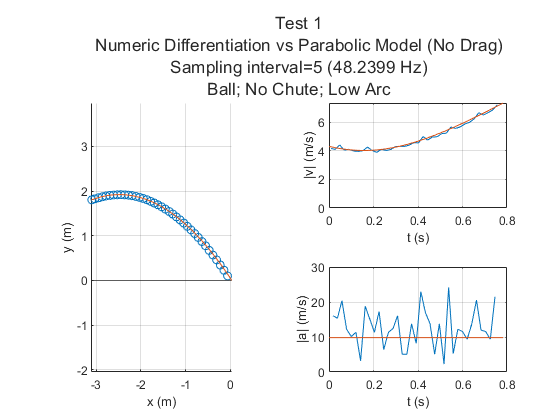
\includegraphics[width=0.9\linewidth]{images/Analysis1_Test1_Fig5_NoDrag.png}
\caption{\label{fig:Analysis1_Test1_Fig5_NoDrag} Fitting the parabolic model to sampled position data for a ball with no parachute. Left: Sampled position (blue) with the fit trajectory (orange). Right: Velocity and acceleration computed using numeric differentiation (blue) and the model's velocity and acceleration (orange). For low-drag scenarios, the parabolic model appears adequate.}
\end{figure}

We started by fitting our parabolic model on some data of just the plain ball with no parachute attached. It was thrown in a low arc; keeping the speed low and minimizing drag effects. This should be the best-case scenario for the parabolic model. The data is shown in Fig.~\ref{fig:Analysis1_Test1_Fig5_NoDrag}. 

At first glance, this model is actually looking pretty decent. There aren't any huge problems with the trajectory plot at this scale. Looking at the numeric differentiation, it's clear that there's plenty of noise in the signal. The velocity plot has some noise, and the model's velocity forms a smooth line through the middle of it. The noise in the signal makes the numeric differentiation's acceleration data nearly useless, but the model's acceleration is a constant 1g as expected. 

This is all good news because it verifies that the code we've been working on up until now works as intended. There certainly was no need for multiple cycles of struggle and debugging.\footnote{This is sarcasm.} In addition to verifying the code, if this projectile had been the only design we cared about, we would probably just call it a day here and save ourselves a lot of work by not implementing the linear drag model. Alas, someone had the bright idea to put a parachute on that ball. Let's look at that data next.


\subsection{Test Case: High Drag}

%% Test 4

\begin{figure}[t]
\centering
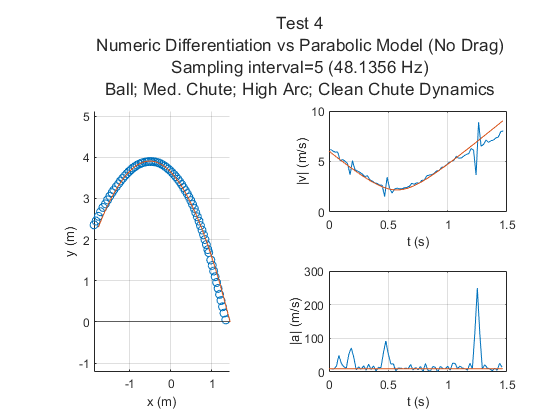
\includegraphics[width=0.9\linewidth]{images/Analysis1_Test4_Fig5_NoDrag.png}
\caption{\label{fig:Analysis1_Test4_Fig5_NoDrag} Fitting the parabolic model to sampled position data for a ball with a parachute. Judging by the position plot, the parabolic model is unable to adequately capture the motion of this system.}
\end{figure}

\begin{figure}[t]
\centering
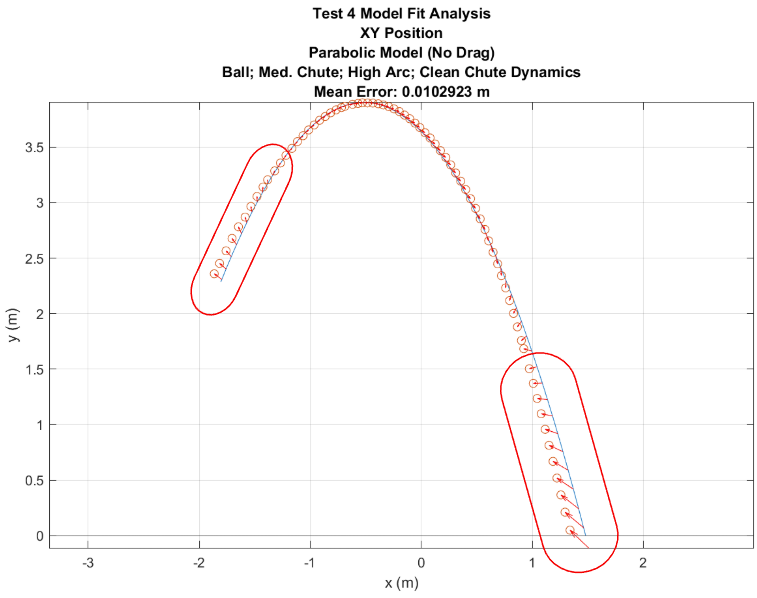
\includegraphics[width=0.9\linewidth]{images/Analysis1_Test4_Err_NoDrag.png}
\caption{\label{fig:Analysis1_Test4_Err_NoDrag} A closer look at the failure of the parabolic model. Red vectors show the error for each sampled position. The highlighted regions at the start and end of the trajectory show how the parabolic model deviates from the observed data.}
\end{figure}

Here the limitations of the parabolic model become more apparent. The data for a higher drag scenario is shown in Fig.~\ref{fig:Analysis1_Test4_Fig5_NoDrag}, and Fig.~\ref{fig:Analysis1_Test4_Err_NoDrag} presents the trajectory in more detail. The model fits decently around the apex, but is way off at the start and end. Clearly, drag plays a more significant role than the parabolic model can account for. 

At this point it's tempting to see the model failing in this way and immediately take this as the justification we need to invest in the linear drag model. But let's do a quick vibe check. What if we didn't expect it to fail like this? Does it make sense that incorporating linear drag would help? After all, it isn't just the drag we increased. Attaching the chute via strings turns this into a complex multibody system. What trajectory would we expect from two point masses attached by spring? Answering these questions is left as an exercise for the reader. We will carry on with the analysis assuming linear drag will be the solution.


\subsection{Test Case: High Drag - Frame by Frame}

\begin{figure*}[t!]
    \centering
    \begin{subfigure}[t]{0.5\textwidth}
        \centering
        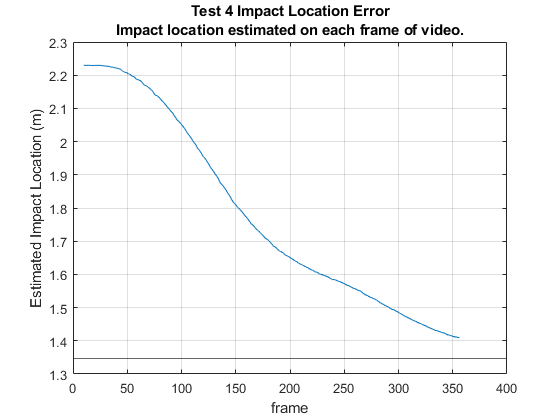
\includegraphics[width=\textwidth]{images/Analysis1_Test4_ImpLocPlot_NoDrag.png}
        \caption{}
    \end{subfigure}%
    ~ 
    \begin{subfigure}[t]{0.5\textwidth}
        \centering
        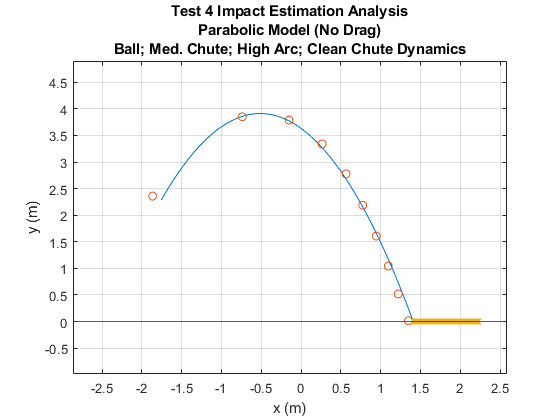
\includegraphics[width=\textwidth]{images/Analysis1_Test4_ImpLocHist_NoDrag.png}
        \caption{}
    \end{subfigure}
    \caption{\label{fig:Test4_NoDrag_FrameByFrame} Frame-by-frame impact location estimation for a ball with a parachute using the parabolic model. (a) Impact location over time. (b) Impact locations marked.}
\end{figure*}

We now consider a form of analysis where we fit a trajectory model to the sampled data frame-by-frame; as sort of an analog to using this tool in real-time. For each frame of video data, we select 10 points spaced between the start of the data up until the current frame. We then fit a trajectory to that subset of the data and record the predicted impact location. This is done for each frame of the video. Results are shown in Fig.~\ref{fig:Test4_NoDrag_FrameByFrame}. 

What becomes immediately apparent is that the estimates derived frame-by-frame failed to align with the observed impact position. Even up to the moment of impact. And it's not just noise, there's clearly some unmodeled behavior causing this offset in the error. There's one clear conclusion that we draw from this: The parabolic model, which completely ignores drag, is simply inadequate for predicting the trajectory when drag is significant. 


\section{Model Refinement - Linear Drag Model}

Now that we are confident in our code architecture and we have proven that the simple parabolic model is inadequate, we can move on to developing the linear drag model. 

By linear drag we mean that, in addition to gravity, there is a new force which is linearly proportional to the projectile velocity and opposite in magnitude. 

\begin{align*}
\vec{F}_{\text{drag}} = -b\vec{v}
\end{align*}

With this drag force, and gravity, the equations of motions are derived by the video linked in the footnote.\footnote{Dr Ben Yelverton - Trajectory of a projectile with linear drag \href{https://www.youtube.com/watch?v=Tr\_TpLk3dY8}{https://www.youtube.com/watch?v=Tr\_TpLk3dY8}} We then used WolframAlpha to evaluate the derivatives for velocity and acceleration, and the final model is as follows:

% Linear Drag Model
\begin{align*}
&Model_{\text{Linear Drag}} = \\
&\begin{cases} 
\displaystyle \ddot{\bf r}(t) = \left[-\frac{1}{m}e^{-bt/m}(b\dot{\bf r}_{0y}+gm)\right]\hat{y} + \left[-\frac{b}{m}\dot{\bf r}_{0x}e^{-bt/m}\right]\hat{x} 
\\
\displaystyle \dot{\bf r}(t) = \left[\frac{1}{b}e^{-bt/m}(b\dot{\bf r}_{0y}+gm)-\frac{gm}{b}\right]\hat{y} + \left[\dot{\bf r}_{0x}e^{-bt/m}\right]\hat{x} 
\\
\displaystyle {\bf r}(t) = \left[\frac{m}{b}(\dot{\bf r}_{0y}+\frac{mg}{b})(1-e^{-bt/m})-\frac{mgt}{b}\right]\hat{y} + \left[\frac{m\dot{\bf r}_{0x}}{b}(1-e^{-bt/m})\right]\hat{x} + {\bf r}_0\\
t_{impact} = t > 0\text{ where }{\bf r}_y(t) = 0
\end{cases}
\end{align*}

where $g=9.81m/s^2$ is the acceleration due to gravity, ${\bf r}_0$ is the initial position, $\dot{\bf r}_0$ is the initial velocity, $\hat{y}$ is the unit vector in the upwards vertical direction, and $\hat{x}$ is the unit vector in the right direction. The projectile mass will be set to $m=1$ and $b$ will be fit by gradient descent.\footnote{We believe setting $m=1$ and fitting $b$ with gradient descent is valid if you're only interested in the projectile's trajectory and not the actual drag coefficient value.} A portion of the code implementation of this model is shown in Fig.~\ref{fig:model_matlab_code_lineardrag}.

\begin{figure}[t]
\centering
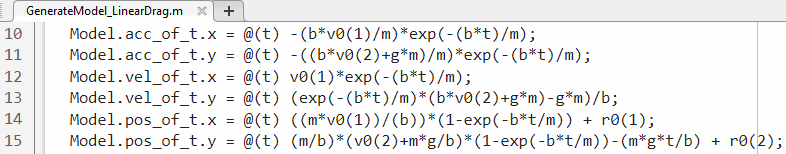
\includegraphics[width=\linewidth]{images/model_matlab_code_lineardrag.png}
\caption{\label{fig:model_matlab_code_lineardrag} Equations of motion for an object experiencing linear aerodynamic drag implemented in MATLAB. Full code available on GitHub.}
\end{figure}

Don't worry about fully understanding those equations too much. None of us did. Just because we know \LaTeX\ doesn't mean we're savants. What we're interested in is if it can form a trajectory that fits better than the parabolic model. If you're a frickin nerd and you \textit{do} want to analyze the math, take a look at the velocity function. Notice there's the exponential decay term of the form $e^{-t}$. For the $y$ component of the velocity, there will be some terminal velocity it reaches. For the $x$ component of velocity, it'll tend to 0. 

Thanks to our modular code architecture, we're able to implement this model as a new function file with no change to the rest of the code architecture. We can run our analysis with either version of the model by just changing an option value.

\section{Results Analysis 2}
\section{Applications and Future Work}

Philosophers have hitherto only interpreted the world in various ways; the point is to change it. By which we mean there's little point in simply analyzing the trajectory without actually using that information to do something useful. Here we'll discuss what some applications of this project might be, and what would need to be worked on to make it a reality.

\subsection{Engineering Applications}
Drag Comparison - This system could be used as-is for comparing drag coefficients between different projectile designs. While this system isn't great for determining the drag coefficient of an object in isolation (because it assumes the mass is 1), it could still be used for comparing the drag of multiple irregularly shaped but equal mass objects. However, a comparison of this nature could be completed with a simpler system so I might consider this an underutilization of our project. 

Gravity Calibration - Suppose you had a system designed to provide a constant vertical force offset to counteract gravity. Such a system might be used if you were developing a robot to fly on Mars, for example. If we tweaked our system to fit the model's gravity parameter, we could use that info to calibrate our gravity offset equipment. 

\subsection{Real-Time Applications}
If we are able to get this code running in real-time, the limits of the applications would be beyond the scope of this paper. Taking real-time position information and predicting the trajectory could be used for anything from missile defense to fruit harvesting, as mentioned in the intro. The following changes would be necessary to enable real-time operations:
\begin{itemize}

\item The 3rd Dimension

Our code only operates in 2 axes currently. It should be quite straightforward to add a second horizontal axis, and that would probably be necessary for most real world applications.

\item Linearization 

Linearizing the error function would allow us to use a linear regression to fit the trajectory, which would be much faster computationally as well as more accurate. It's possible the current algorithm might run in real-time with enough compute, but optimizing the algorithm with linearization would allow the application to be embedded in a wider variety of hardware.
 
\item Data input stream 

We are currently reading in data by opening a file and reading all the contents at once. To run in real time we might first start by modifying the code to use something like a serial interface. A separate issue would then be what hardware and software to use to generate the position data in real time, since Tracker doesn't do that. MATLAB does have computer vision toolboxes available, so that's something to look into.

\item Data output stream.

Similar to the data input, we'd need a data output. The output content could simply be the impact location, or maybe it's the model parameters. Perhaps another serial stream would do the trick. That would then need to be processed by some other system that can use that information to control actuators to accomplish some desired task. 

\item Miscellaneous Algorithm Tweaks

To account for unmodeled dynamics, tweaks are constantly made to the algorithm. One tweak could be to weight the error terms for the fitting process more strongly if they're more recent data.

\end{itemize}

\section{Error Sources}

Throughout this process there have been several opportunities for inaccuracies to sneak in. 

\TODO
\section{Questions}

Several questions have been asked by our peers in response to the presentation accompanying this report. Some of the Q\&A has been copied verbatim here.

\medskip 

\textit{Why do you suspect the deviation happened more around the beginning and end of the trajectory, whereas the data around the middle appeared to follow the parabolic path?}

\smallskip

The effects of drag are less pronounced at lower velocities, and the apex of the trajectory experiences the lowest velocity. I think this is why the parabolic model fits best near the apex. Additionally, even with drag in the model there are still unmodeled dynamics from the way the parachute interacts with the ball. The parachute sort of oscillates around in a way I didn't anticipate during planning. 

\medskip 

\textit{Did you have a method of standardizing your physical experiments, such as having the same person throw the mass from (approximately) the same location every time?}

\smallskip

Yes, we had Richard write up a test procedure that we followed during filming to keep our tests standardized. We also had tape marked on the floor and predefined thresholds for where the projectile had to land to qualify it as a valid throw. The filming location itself (well lit, lots of right angles, solid color background) was also chosen to help standardize the process.


\medskip 

\textit{I know you mentioned having a lot of sources for error, which do you think impacted your data the most?}

\smallskip

One of the challenge with Tracker is that the automatic tracker (as opposed to manually tracking it frame by frame) will drift away from the center of mass of the tracked object. I manually correct that drift every few frames, and this shows up as spike in the velocity plot and an even larger spike in the acceleration plot. That's probably the most noticeable source of error within the context of the project. If we integrated this work into a larger system, other error sources would become more important.

\medskip 

\textit{Would your data have been more accurate if you used a camera with higher frames to capture more moments and give a more accurate representation of the trajectory since you wont miss a single small detail?}

\smallskip

A higher framerate camera would have reduced the motion blur in the video, allowing us to have higher quality (less noise) input data. That definitely would have helped. However, the sampling rate itself wasn't the deciding factor in accuracy. We actually downsample the data for the majority of the processing to speed up computation. 

If our model treated the ball and parachute as a multibody system then the answer might be different, but as a point mass either with or without drag I think the 240fps sampling rate of our camera was adequate. 

\medskip 

\textit{How did you guys choose the CSUN gym as a place for physical tests?}

\smallskip

We first discussed some general filming location requirements, such as the lighting, background, overall space, and reference features. We came up with a few ideas, including the handball courts. Then a couple team members scouted the location and took photos of the area and put them on Google Drive so we could review them. Once the photos were reviewed and we agreed the location looked good we developed our procedure to use the court specifically (taking advantage of the patterns on the ground, etc). 

\medskip 

\textit{since you tested multiple parachute designs and varied the launch conditions, did you notice any patterns in how certain parachute shapes responded to directional changes in the throw? For instance, did some designs tend to veer off course or rotate more depending on the launch direction? Additionally, how did these behaviors show up in the Tracker software, were they easy to detect, or did they create challenges in accurately capturing the motion?}

\smallskip

We tested multiple different sizes of parachute, but they all had the same basic conical design. The behavior of the chutes was quite variable even among different throws with the same chute, so it's hard to draw conclusions between different chute designs. The larger parachute (we used 3 sizes in total) produced noticeably more drag than the smaller ones. The unmodeled dynamics were definitely larger in magnitude with the larger chute, but if I recall correctly they were roughly of the same nature.  

An example of some unmodeled behavior includes how the strings on the chute go slack during the apex of the trajectory, and then how the chute whips around when the ball starts to fall again. This behavior happened for both the small and large chutes, but has a larger magnitude on larger chutes. 

In Tracker we tracked the chutes as a second body (this data wasn't shown in any of the plots). We attempted to correlate the chute position to the angle, but didn't produce any results clear enough to include in the presentation. 

\medskip 

\textit{Are there ways to implement bounce and possibly predict that?}

\smallskip

Yep! The simplest way to model bounce would be to simply flip the vertical component of the velocity when it impacts the ground. You could also incorporate a coefficient of restitution to model energy lost in the bounce. It would be more complicated if you wanted to model a spinning object hitting the ground. 

\section{Acknowledgments}

The lead author Jaiden would like to thank his co-authors for their support, their interest in learning, and their willingness to try obnoxious new things like \LaTeX and GitHub. We would all like to thank Dr. Maya Pishvar for the opportunity to develop our skills performing Numerical Analysis of Engineering Systems.

\section{Conclusion}

Remind the reader how frickin amazing and wonderful the world is and how the time we live in is so exciting.

Remind them how mind blowing it is that we can see through the noise like in Fig.~\ref{fig:Analysis2_Test4_Fig5_LinearDrag} by leveraging our knowledge of the underlying system mechanics. 

\TODO
\section{References}

\paragraph{Equation of Motions Derivation} 

Dr Ben Yelverton - Trajectory of a projectile with linear drag

\href{https://www.youtube.com/watch?v=Tr\_TpLk3dY8}{https://www.youtube.com/watch?v=Tr\_TpLk3dY8}

\paragraph{GitHub Repository} 

Complete source code for the project. 

\href{https://github.com/JaidenK/ME309\_Spring2025\_Project}{https://github.com/JaidenK/ME309\_Spring2025\_Project}

\paragraph{Tracker} 

Open-source software tool for performing motion tracking and analysis on video files.

\href{https://opensourcephysics.github.io/tracker-website/}{https://opensourcephysics.github.io/tracker-website/}

\section{MISC (Remove before submitting)}


\newpage
% Linear Drag Model
\begin{align*}
\begin{cases} 
\displaystyle \ddot{\bf r}(t) = \left[-\frac{1}{m}e^{-bt/m}(b\dot{\bf r}_{0y}+gm)\right]\hat{y} + \left[-\frac{b}{m}\dot{\bf r}_{0x}e^{-bt/m}\right]\hat{x} 
\\
\displaystyle \dot{\bf r}(t) = \left[\frac{1}{b}e^{-bt/m}(b\dot{\bf r}_{0y}+gm)-\frac{gm}{b}\right]\hat{y} + \left[\dot{\bf r}_{0x}e^{-bt/m}\right]\hat{x} 
\\
\displaystyle {\bf r}(t) = \left[\frac{m}{b}(\dot{\bf r}_{0y}+\frac{mg}{b})(1-e^{-bt/m})-\frac{mgt}{b}\right]\hat{y} + \left[\frac{m\dot{\bf r}_{0x}}{b}(1-e^{-bt/m})\right]\hat{x} + {\bf r}_0
\end{cases}
\end{align*}
where ${\bf r}_0$ is the initial position and $\dot{\bf r}_0$ is the initial velocity. We will set $m=1$ and $b$ will be fit by gradient descent.

\begin{align*}
\text{velocity} = \frac{\Delta \text{position}}{\Delta \text{time}}
\end{align*}

\end{document}
